\documentclass{pracamgr}

\usepackage{polski}

\usepackage[utf8]{inputenc}
\usepackage[T1]{fontenc}
\usepackage{algorithm}
\usepackage[noend]{algpseudocode}
\usepackage{amsmath}
\usepackage{graphicx}
\usepackage{tikz}
\usepackage{verbatim}

\usetikzlibrary{arrows}


\author{Bartosz Marcinkowski}

\nralbumu{319476}

\title{Sztuczna inteligencja na przykladzie gry Quoridor}
\tytulang{Artificial intelligence for the Quoridor game}

\kierunek{Informatyka}

\opiekun{prof. Jana Madeya}

\date{Maj 2016}

\dziedzina{11.3 Informatyka}

\klasyfikacja{
I. Computing Methodologies \\
  I.2. Artificial intelligence \\
  I.2.1. Applications and Expert Systems}

\keywords{
	sztuczna inteligencja, gry planszowe
}

% Tu jest dobre miejsce na Twoje własne makra i~środowiska:
\newtheorem{defi}{Definicja}[section]

% koniec definicji

\begin{document}
\maketitle

\begin{abstract}
TODO
\end{abstract}

\tableofcontents
%\listoffigures
%\listoftables


\chapter{Wprowadzenie}

W pracy zajmiemy się sztuczną inteligencją dla gry Quoridor. W dalszej części pierwszego rozdziału opiszemy zasady gry w wersji oryginalnego wydawcy i wskażemy istniejące niedoskonałości, określimy założenia i oczekiwania wobec tej pracy i dokonamy przeglądu istniejących rozwiązań, aby uzasadnić podjęcie tematu. W drugim rodziale dokonamy przeglądu ogólnych metod szcztucznej inteligencji używanych do implementacji graczy komputerowych. W trzecim rozdziale rozstrzygniemy kwestię zasad gry. W czwartym opiszemy i uzasadnimy wybór technologii użytych do implementacji i porównywania rozważanych później algorytmów. W piątym rozdziale opiszemy proces rozwijania kolejnych algorytmów, aż w końcu w szóstym podsumujemy efekty naszej pracy.

\section{Quoridor - oryginalne zasady gry}

Gra rozgrywa się na planszy za pomocą 4 pionków i 20 ogrodzeń, nazywanych też ścianami. Na planszy znajduje się siatka szczelin wyznaczająca 81 kwadratowych pól, tworzących układ 9~x~9. Każdy pionek ma unikatowy kolor, mieści się na jednym polu planszy i nie może go dzielić z innym. Ogrodzenia są identyczne i dają się umieszczać w szczelinach między polami planszy. Ogrodzenie jest dwukrotnie dłuższe od boku pola, więc (poprawnie umieszczone) sąsiaduje z dwoma polami z każdej strony, zajmuje całą szerokość szczeliny i jedno skrzyżowanie szczelin.

W grze może wziąć udział dwóch lub czterech graczy. W obu przypadkach otrzymują po jednym pionku, dzielą się po równo ogrodzeniami i przypisują się do różnych boków planszy; jeżeli jest ich dwóch, muszą to być boki przeciwległe.

Na początku gry na planszy nie ma ogrodzeń (stanowią zasoby graczy), a pionek każdego gracza umieszcza się na polu przy środku boku, do którego jest przypisany.
Następnie gracze wykonują kolejno swoje ruchy. Celem gry jest dotarcie swoim pionkiem do boku planszy przeciwległego wobec boku, do którego jest się przypisanym. Gra kończy się w momencie, w którym jednemu z graczy się to uda.

Każdy ruch może polegać na ustawieniu jednego ze swoich nieużytych ogrodzeń na planszy albo przesunięciu pionka. Ogrodzenie nie może kolidować z żadnym innym i nie może odciąć żadnemu graczowi wszystkich dróg do celu. Ruch pionkiem polega na przesunięciu go na puste, sąsiadnie pole (sąsiedztwo wyznacza wspólny bok).

Jeżeli na pewnym sąsiednim, nieodgrodzonym polu znajduje się już pionek przeciwnika, można wykonać skok na pole za tym pionkiem, o ile jest ono puste i nieodgrodzone. Jeżeli taki skok nie jest możliwy, można wykonać skok na jedno z dwóch pozostałych pól sąsiadujących z przeciwnikiem, znów o ile jest puste i nieodgrodzone.

\section{Niedoskonałość oryginalnych zasad}

Dla pewnych stanów gry oryginalne zasady nie odpowiadają jednoznacznie na pytanie o legalne ruchy albo dają odpowiedź nieoczekiwaną, wyglądającą na efekt niedopatrzenia. Możliwe, że autorzy i wydawcy gry świadomie woleli pozostawić mało prawdopodobne sytuacje do rozsądzenia graczom niż wydłużać instrukcję analizami kolejnych przypadków, jednak w przypadku tej pracy takie podejście jest niedopuszczalne. Automatyczne testowanie algorytmów sztucznej inteligencji zwiększa prawdopodobieństwo natrafienia na problematyczne stany gry, co może zaburzyć wynik pracy. W tym miejscu zarysujemy tylko problem przykładem, odkładając rozważania nad możliwymi rozwiązaniami na dalszą część pracy.

\subsection*{Brak legalnych ruchów}

Niech pionki czarny i zielony sąsiadują z pionkiem czerwonym. Dalej, niech pionek czarny będzie odgrodzony od wszystkich sąsiednich pól oprócz tego, na którym stoi czerwony i niech czerwony będzie odgrodzony od tych pól, na których nie stoją czarny ani zielony. Teraz, jeżeli właściciel pionka czarnego nie ma już ogrodzeń, nie może wykonać ruchu.

\begin{figure}[ht!]
\centering
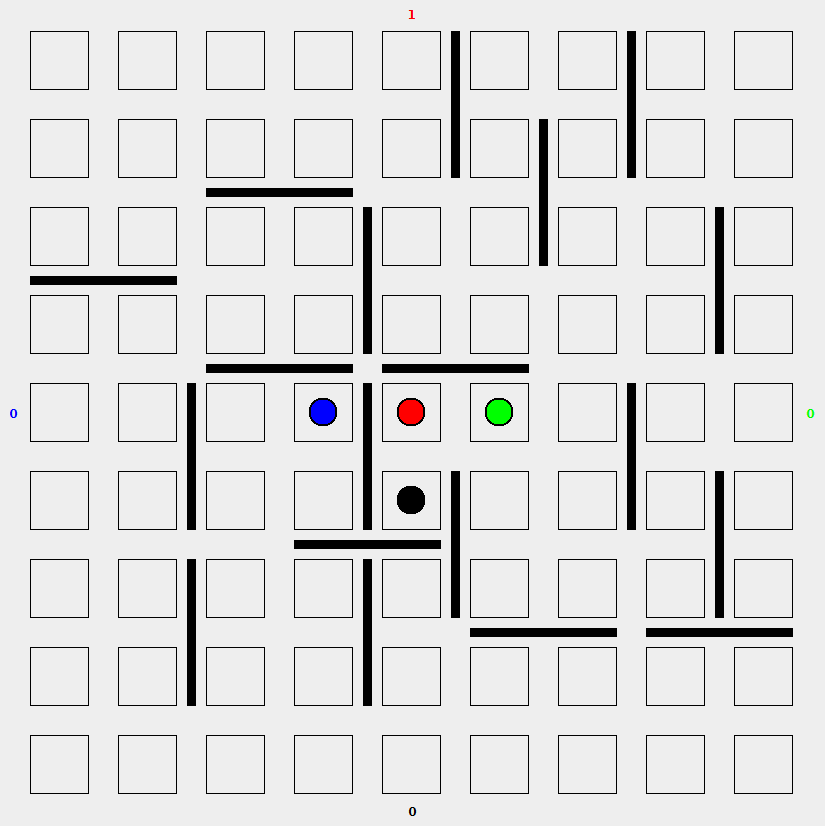
\includegraphics[width=120mm]{img/no-move.png}
\caption{Brak legalnych ruchów \label{overflow}}
\end{figure}

\section{Cele i założenia}

Opracowywanie graczy sterowanych komputerowo do gier planszowych może mieć różne założenia i cele. Pełne rozwiązanie gier z dużą ilością stanów wymaga mocy obliczeniowej przekraczającej możliwości komputera osobistego, a nawet jeśli uzyska się je na superkomputerze, to wynikowa tablica optymalnych ruchów nie nadaje się do dystrybucji wraz z grą. Celem tej pracy jest opracowanie algorytmów sztucznej inteligencji dla gry Quoridor i utworzenie oprogramowania open-source, łatwego w dystrybucji i nadającego się do użycia na komputerze osobistym lub urządzeniu przenośnym, które będzie umożliwało grę człowieka przeciwko różnym algorytmom, obserwowanie rozgrywek między graczami komputerowymi oraz porównywanie graczy komputerowych poprzez przeprowadzanie automatycznych turniejów (w tym ostatnim przypadku bez interfejsu dla użytkownika).

Dodatkowo chcielibyśmy rozwiązać problem responsywności gracza komputerowego, który pojawia się w wielu aplikacjach. Mianowicie chcielibyśmy uniknąć rozwiązań, w których czas działania algorytmu jest regulowany parametrem specyficznym dla danego algorytmu sztucznej inteligencji, np. głębokością przeszukiwania drzewa stanów gry, i dopiero po wykonaniu całego algorytmu zwracany jest wynik. Takie rozwiązania nie gwarantują w rzeczywistości żadnego ograniczenia na czas w jakim komputer wykona ruch. Zamiast tego, chcielibyśmy zaprojektować algorytmy w taki sposób, żeby w można było przerwać ruch gracza komputerowego w dowolnym momencie, uzyskując decyzję o ruchu, który wydawał się optymalny w podczas przerwania obliczeń, i jednocześnie nie uzyskać algorytmu silnie uzależnionego od czynników losowych, jak np. kolejność rozpatrywania dopuszczalnych ruchów.

\section{Istniejące rozwiązania}

Wśród projektów open-source dotyczących gry Quoridor, które znaleźliśmy, żaden nie zawiera zadowalającego algorytmu sztucznej inteligencji. Są to albo serwery gry, zajmujące się wyłącznie przestrzeganiem zasad gry i pozostawiające wybór ruchu poza zakresem projektu, albo aplikacje pozwalające grać z naiwnym graczem komputerowym. Nie widać też w prób rozwiązania problemu responsywności.

\chapter{Podstawowe metody sztucznej inteligencji dla gier}

Istnieją standardowe, ogólne metody tworzenia algorytmów sztucznej inteligencji graczy komputerowych, które korzystają z podobnych założeń i abstrakcji. W tym rozdziale opiszemy te założenia i metody, a później odniesiemy je do gry Quoridor i przyjętych wcześniej założeń.

\section{Podstawowe pojęcia}

Algorytmy, które tu przedstawimy, dotyczą deterministycznych gier dla dwóch graczy, o sumie zerowej, z pełną informacją o stanie gry, w których gracze wykonują ruchy na zmianę. Suma zerowa oznacza, że wygrana jednego gracza oznacza przegraną drugiego.

Podstawową abstrakcją używaną do reprezentacji gry jest graf skierowany, w którym wierzchołki reprezentują stany gry, a krawędzie reprezentują legalne ruchy. Rozgrywka jest reprezentowana przez ścieżkę, być może zawierającą cykle, od wierzchołka reprezentującego stan początkowy do jednego z wierzchołków reprezentujących stan końcowy.

Na potrzeby algorytmów sztucznej inteligencji często wygodniej jest użyć drzewa gry, w którym wiele wierzchołków może reprezentować ten sam stan gry. Stan początkowy jest reprezentowany korzeniem, stany końcowe liśćmi a rozgrywka ścieżką od korzenia do liścia.

W dalszej części pracy będziemy zamiennie używać pojęć stan i wierzchołek, ruch i krawędź itd. o ile nie będzie powodować to nieporozumień.

Kolejnym pojęciem pojawiającym się w tych algorytmach jest funkcja oceniająca. Jest to funkcja przypisująca stanowi gry liczbę całkowitą, która ma oceniać jak bardzo pożądany jest ten stan dla dangego gracza. Powinna przyjmować skrajne wartości dla stanów końcowych (największą dla wygrywających, a najmniejszą dla przegrywających).

\section{Minimax i Alfa-Beta}

\subsection{Minimax}

Algorytm Minimax nazywa graczy \(min\) i \(max\) oraz rozpatruje w drzewie gry tylko poddrzewo bieżącego stanu gry do ustalonej głębokości. W tak uzyskanym drzewie liściom przypisana jest wartość funkcji oceniającej dla gracza \(max\). Pozostałe wierzchołki będą miały przypisywane wartości na podstawie wartości synów.

Wobec definicji funkcji oceniającej oczekujemy, że gracz \(max\) zawsze wybierze ruch prowadzący do syna o największej wartości, więc w grze o sumie zerowej gracz \(min\) będzie wybierał najmniejsze wartości. Zatem wartości \("minimax"\) dla wszystkich wierzchołków możemy obliczyć następująco:

\begin{algorithm}
\caption{minimax}\label{minimax}
\begin{algorithmic}[1]
\Function{minimax}{$v$}
\If {$jestLisciem(v)$}
	\State \Return $funkcjaOceniajacaDlaGraczaMax(v)$
\EndIf
\If {$aktualyGracz(s) == graczMax$}
	\State \Return $max$($minimax(s) | s \in synowie(v))$
\Else
	\State \Return $max$($minimax(s) | s \in synowie(v))$
\EndIf
\EndFunction
\end{algorithmic}
\end{algorithm}

Znając wartości \(minimax\) dla synów korzenia, możemy wybrać najkorzystniejszy ruch w obecnym stanie gry.

\subsection{Alfa-Beta}

Algorytm Alfa-Beta jest ulepszeniem algorytmu minimax. Opiera się na następującej obserwacji: wartości \(minimax\) niektórych wierzchołków mogą być ustalone bez obliczania ich dla wszystkich potomków aż do liści, a więc niektóre obliczenia poprzedniego algorytmu są zbędne. Oszczędzając w ten sposób czas można zwiększyć głębokość przeszukiwanego drzewa, a więc podjąć lepszą decyzję.

Poniższe drzewo ilustruje sytuację, w której po obliczeniu wartości \(minimax\) dla części wierzchołków drzewa można stwierdzić jaka jest wartość korzenia.

\begin{center}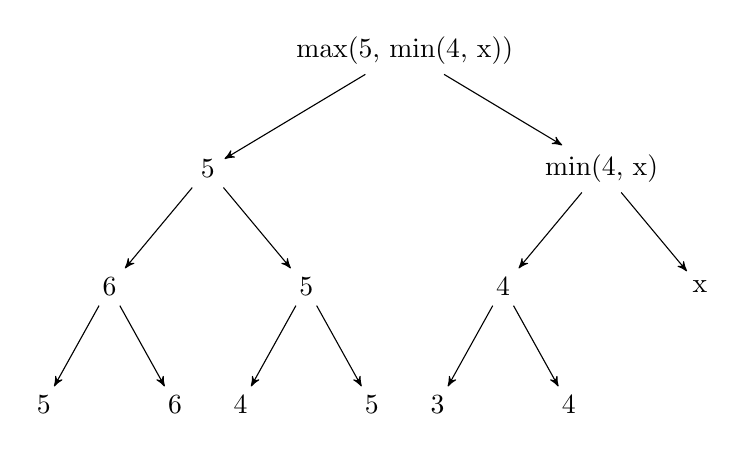
\begin{tikzpicture}[->,>=stealth',level/.style={sibling distance = 5cm/#1,
  level distance = 1.5cm}]
\node {max(5, min(4, x))}
    child{ node {5}
    	child{ node {6}
            child{ node {5}}
            child{ node {6}}
        }
		child{ node {5}
            child{ node {4}}
            child{ node {5}}
        }
    }
    child{ node {min(4, x)}
        child{ node {4}
            child{ node {3}}
            child{ node {4}}
        }
        child{ node {x}}
    }
;
\end{tikzpicture}
\end{center}

\subsection{Dalsze ulepszenia}

TODO tablica transpozycji, MTD-f, NegaScout, PVS

\section{Metody Monte Carlo}

TODO

\section{Odniesienie przedstawionych metod do tej pracy}

TODO

\begin{thebibliography}{99}
\addcontentsline{toc}{chapter}{Bibliografia}
\end{thebibliography}

\end{document}


%%% Local Variables:
%%% mode: latex
%%% TeX-master: t
%%% coding: utf-8
%%% End:
